\documentclass{article}

\usepackage{graphicx}
\usepackage{hyperref}
\usepackage{listings}
\usepackage{parskip}

% Listings configuration

\lstset{tabsize=2}

\title{Improving search for Packagist}

\author{Bert Peters --- s1147919}

\date{Multimedia Information Retrieval, spring 2017}


\begin{document}

\maketitle

\begin{abstract}
	In the last few years, PHP as a development platform has been through some large changes. One of the key reasons for this is the emergence of Composer package manager, and its central package repository Packagist. Using these tools, library interoperability is easier than ever before.

	However, library discovery is still hard, with the search functionality of the Packagist being rather lacking, with a very broad text search and a counterintuitive ordering. In this paper, we create a new search engine for Packagist with improved text search and better ordering using pagerank.
\end{abstract}

\section{Introduction}

\section{Related work}

\section{Implementation}

Our implementation consists of 4 main parts, a \emph{downloader} for getting all data off Packagist, an \emph{indexer} to create the search index, a \emph{ranker} that commputes the relevance of each package, and a \emph{searcher} to get the final search results. We also include a simple front end for the searcher, but that component is optional. In the following sections, we will discuss each of these components in more detail. A more usage-specific introduction can be found in the project's README.

For our data structure, we opted to use flat files using filenames as our indexing mechanism. This gives reasonable performance at very little implementation cost.

\subsection{Downloader}

We retrieve a list of packages and the meta-data for all packages from Packagist, using their API~\cite{packagist-api}. We parse the responses using the Jsoncpp library. Overall, we do 1 HTTP request to retrieve the list of packages, and then one more for each individual package. All versions are retrieved at once.

While the above means that we will be hitting the API over 200,000 times, but since all responses are cached to static files, local disk will likely be a more severe bottleneck in performance and slow us down enough not to be a hassle to the remote server.

\subsection{Indexer}
\label{sec:indexer}

In order for our searcher to be fast and accurate, we create an index on our dataset. We use 3 indices: 2 keyword based indices for the package description and package keywords, and a reverse dependency index. Additionally, we create a file containing a list of all valid packages.

For the keyword indices, we create a file for each keyword, and in it write the name of every package that references that keyword. For its name we use the (hexadecimal) MD5 hash of the filename, in order to avoid weird issues with invalid names. We use OpenSSL implementation of MD5 for this, since it is available on most systems.

The reverse dependecy index uses a similar approach, where we have a file for each package\footnote{Note: for efficiency we only create a file for packages that actually have dependents, which is about a third of the total.} and in it we have the list of packages that depend on it. Here we also hash the package name to get a filename. As a consequence of the way we index packages, each index happens to be sorted. We use this for the searching part.


\subsection{Ranker}

There are various metrics that could be used for the relative importance of a package. Packagist provides several; for example the number of downloads in the past week, or the number of stars its Github repository has. Both have its flaws; some packages have hugely inflated download counts due to continuous integration builds, and buying Github stars is not unheard of.\footnote{A quick Google search brings you to \url{http://githubstars.com/}, which apparantly sells exactly this.}

Instead of using one of the provided metrics, we instead opted to use a package's pagerank~\cite{pagerank}
in the dependency graph. In this graph, each package is a node and a directed edge from $a$ to $b$ exists if $a$ depends on $b$. For these purposes, we ignore version constraints, and group all the dependencies of all packages together.

The rationale behind this is the same as with the download count: more people use it, so it is probably more important. However, in contrast to the download count, it is influenced less by CI systems. This system too could be gamed, by uploading countless dummy packages that depend on your main one, but this is easily discovered, and not currently a problem.

Computing the actual pagerank is relatively cheap, since a dependency contains very few cycles~\footnote{Intuitively, there should be no cycles, but there are some split-up libraries where some parts depend upon each other.} and the pagerank stabilizes almost immediately. Rather than implementing pagerank ourselves we use the NetworkX~\cite{networkx} Python library to do this for us. We then save the resulting weights in a file, sorted on package name.


\subsection{Searcher}

Our search component takes a search request, and then prints a newline-delimited ordered list of packages to the standard output. We chose to use Json files as our input for queries, since we can easily express complicated queries in it, and do not have to do complicated command-line escaping to communicate. A sample of our format is shown below:

\lstinputlisting{../search-sample.json}

Here we see a list of terms, which each have a word they look for, and a type which indicates which index will be looked into. Both \texttt{keyword} and \texttt{description} use the keyword indices described in the previous section, and \texttt{name} does a substring match on the name of the package. All types can occur multiple times.

Additionally, we see the \texttt{conjunctive} option, which is optional and can specify whether a result needs to match all predicates (false, default) or any.

Efficiency is paramount for this component since it needs to happen in real time. For the following section, we are going to assume that the time to read a package name is constant, that we have $m$ packages in our data set, and that we have $n$ results for a query and $k$ terms in total. It should be noted that by necessity, $m \geq n$.

The keyword searches are simply reading in a file and returning all $n$ matching packages. Consequently, it is simply $O(n)$. Searching on the name requires reading in all the package names, and performing a substring search on each of them. This is a linear operation on a constant bounded size, since package names are typically limited in length. Thus, the only real complexity here is $O(m)$, reading in all packages.

We process each search term individually, and then combine them. As mentioned in \autoref{sec:indexer}, all of our indices are sorted and thus produce sorted result lists. We can then combine each pair in $O(n_1 + n_2)$ time, both conjunctively and disjunctively, using C++ standard library algorithms. This is still linear in the number of results.

Using the above, it is easy to see that we have an upper bound of $O(km)$ for constructing the result set.

For ranking results, we need to match each package to its rank number. We can do this in $O(m)$ time by using the fact that both the resultlist and the ranklist are sorted, iterating over the latter and advancing the first upon matching. Then we can finally sort the list in $O(n \log n)$ using any sorting algorithm\footnote{We use the sorting algorithm from \texttt{glibc} which is a variation on quicksort, but any algorithm will do.} and output the result.

\subsection{Search front-end}

For the purpose of testing, we created a simple web front-end for our search engine in PHP. A screenshot of it can be seen in \autoref{fig:screenshot}. It includes all three search term types, and each field will be split into more keywords as needed.

The results are shown with their description fields, as well as their latest stable version, if applicable. For comparing versions, we use Composer itself, and the mark-up is slightly enhanced with Twitter Bootstrap, both installed using composer.

\section{Analysis}

In this section, we will discuss some details about the retrieved data, and compare some results between the native Packagist search and our own search.


\begin{figure}
	\centering
	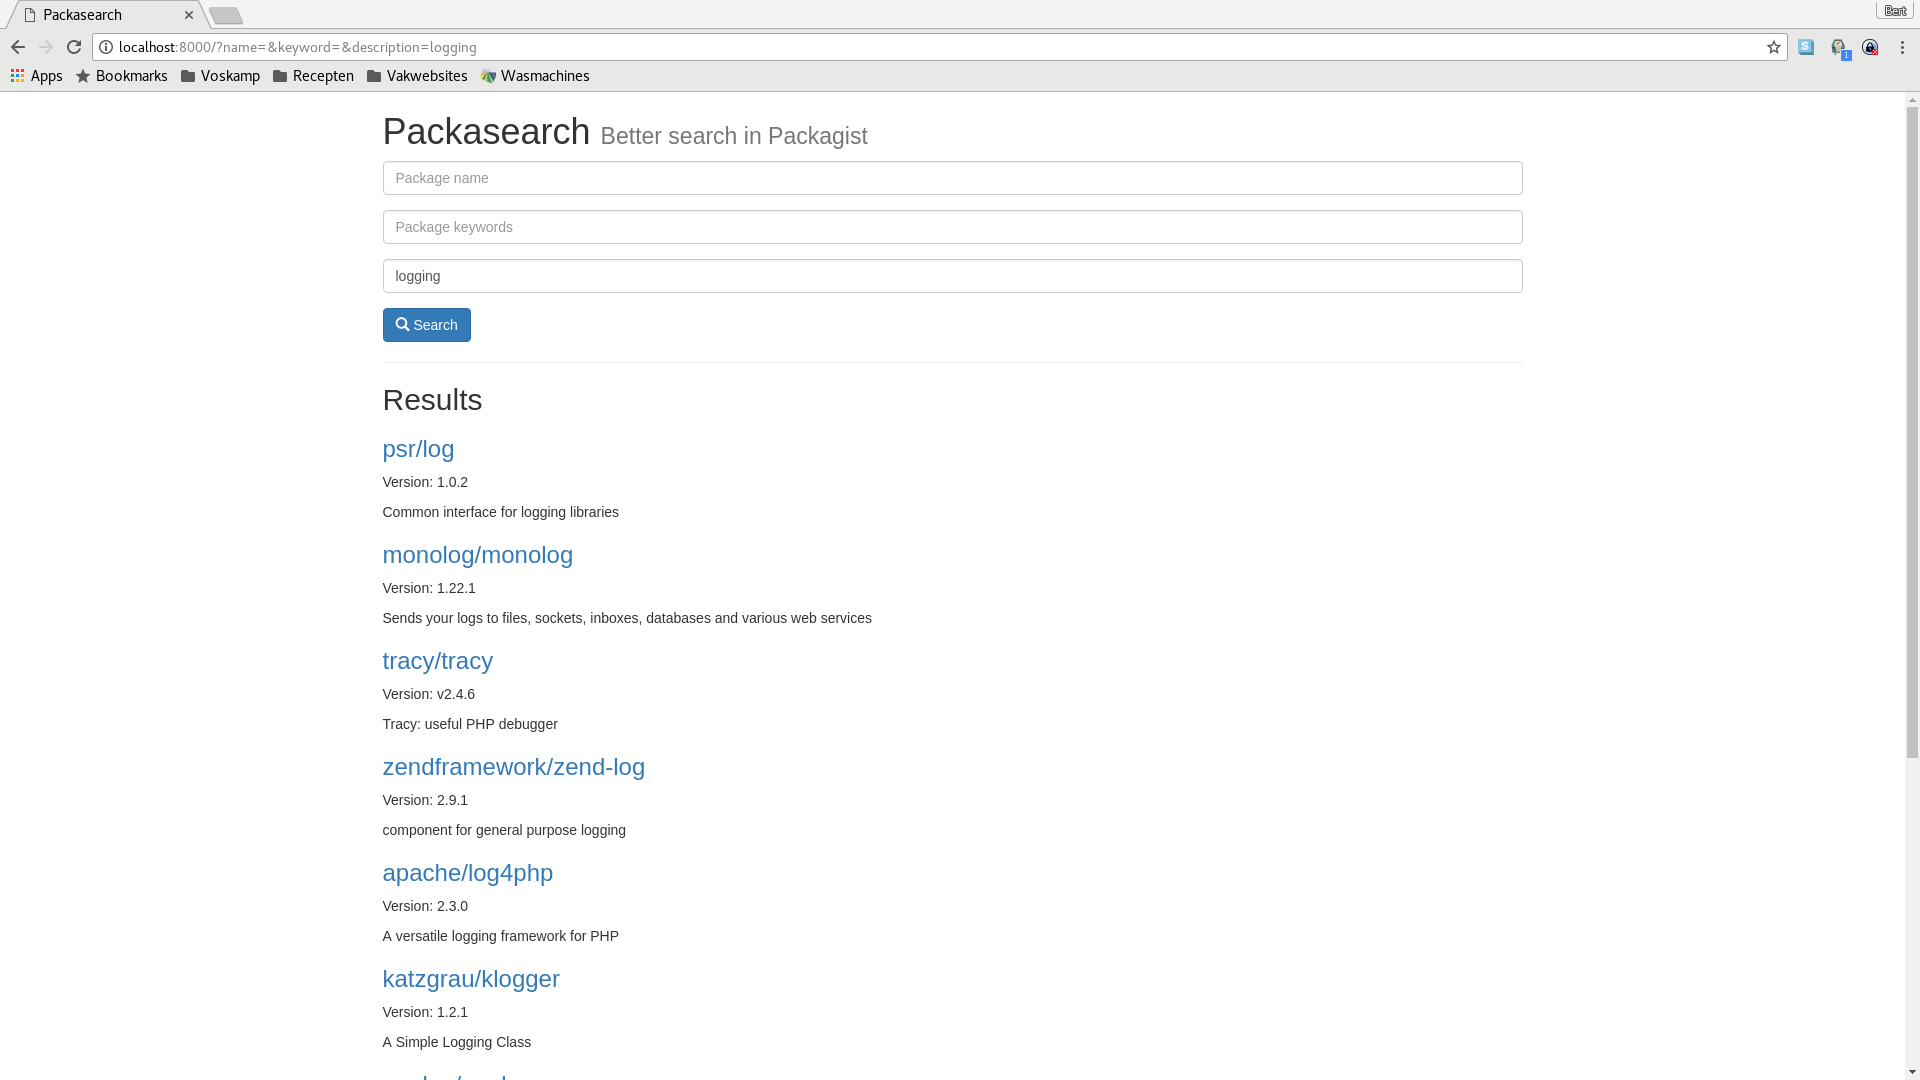
\includegraphics[width=\textwidth]{screenshot}
	\caption{Screenshot of the search front-end}
	\label{fig:screenshot}
\end{figure}

\subsection{Dataset}

\begin{figure}
	\centering
	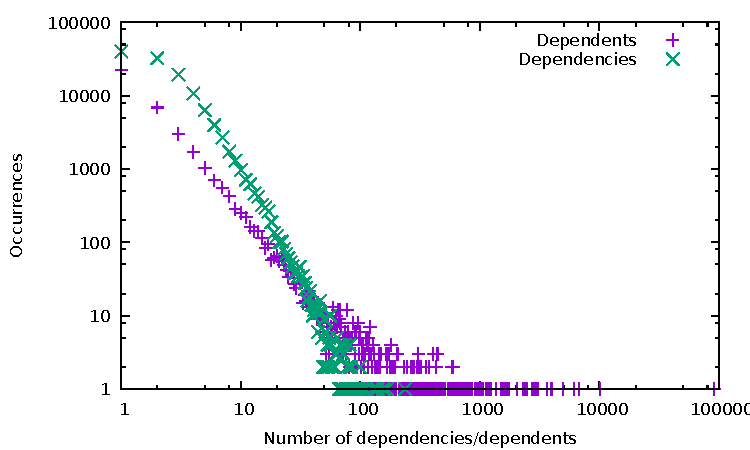
\includegraphics[width=\textwidth]{dependencies}
	\caption{Distribution of number of dependents/dependencies}
	\label{fig:dependencies}
\end{figure}

The first thing we did to verify our hypothesis that the dependency graph would be a good indicator of relevance, is look at the distribution of dependencies and dependents. A visualisation of this is shown in \autoref{fig:dependencies}.

What we see is that there is one package on which nearly half all packages depend. This is because you can list PHP itself as a dependency to declare compatibility. It is also possible to require PHP extensions this way, and about 1\% of packages has cURL as its dependency.

The package with the most dependencies is Drupal, a PHP content management system. It has moved to composer a few years ago, and has since been split up in submodules of its original form. Of its 236 dependencies, 198 are Drupal parts.

\begin{figure}
	\centering
	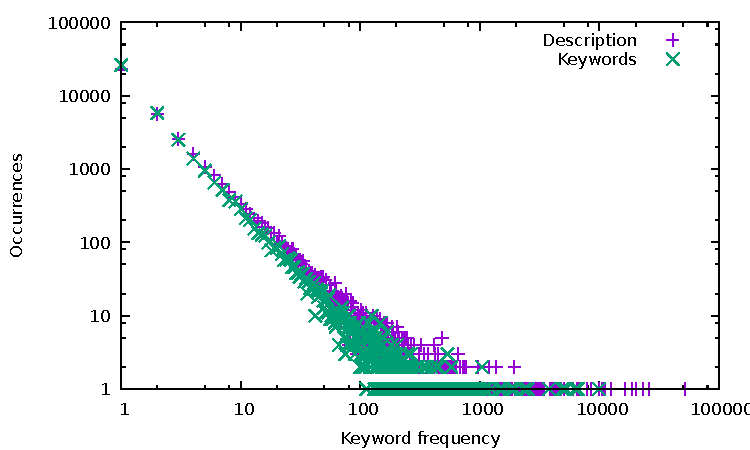
\includegraphics[width=\textwidth]{keywords}
	\caption{Distribution of frequency of keywords}
	\label{fig:keywords}
\end{figure}

Another thing we looked at was the relative frequency of the keywords, of which the distribution can be seen in \autoref{fig:keywords}. Unfortunately, the index does not contain enough information to reconstruct the common words (other than reversing MD5 hashes) but the general distribution appears to be power-law like, which is common in natural language~\cite{zipf}.

\subsection{Search comparison}

For this section, we look at a two case studies for common library searches. In each case, we want to find certain packages, and compare the results for both.

\subsubsection{Templating}

In this case, we want to find a templating library for PHP, to avoid interspersing PHP and HTML\footnote{Which, coincedentally, our search front-end is riddled with.}. In this case, we look at both the description and keyword field, since a name doesn't say much about what it does. On packagist, we just type ``template'' into the search bar.

We should find references to Twig and Smarty, the current and former leading libraries in this area. Searching by tag, we don't find either, but do find Latte, which is popular as well, and we find some libraries interacting with Twig. Using the description field, we find both as our first two results, which is nice.

Using packagist we find neither (at least not on the first page) and the only remotely popular one is the templating engine included in the PHPixie framework. It seems however that Packagist does a substring search on the description, while prefering exact keyword results if available. When we use the keyword ``templat'' rather than ``template'' we do find both.

\subsubsection{Logging}

We want to find a nice logging library to suit our needs. The most important things are \texttt{psr/log} and Monolog, the unofficial logging library interface standard and its most popular implementation respectively. In our search engine, both show up for the keyword ``log'' and for keyword/description ``logging''.

In Packagist, we always find \texttt{psr/log}, but Monolog only shows up for ``loggi''. We suspect that this is once again because of the substring search in the description.


\section{Conclusion}

We have created a fully functional search engine for the Packagist package repository, and compared it to the currently available search system. We found we have comparable, or slightly better results. The existing system is sometimes slightly still better, as its substring search on the description appears to be very useful in various corner cases.

Performance wise the system is up to par, as the results are as instant here as they are for the existing search. An interesting experiment would be to implement the instant-search of the packagist website and see how well that wors.


An area that still needs the most improvement, is the interface. Our current mock-up works, but it might be more user-friendly to take one kind of search terms, and then intelligently split over the various indices. That topic will need further research.

\bibliography{bibliography}{}
\bibliographystyle{plain}

\end{document}
